\documentclass[lualatex,hyperref={pdfencoding=auto}]{beamer}
\usepackage[czech]{babel}
\usepackage{tikz}
\usetikzlibrary{positioning,calc}
\usetheme[fei]{vsb}

\title[Komprese stromových struktur]{Komprese stromových struktur}
\subtitle{Semestrální projekt}
\author{Marek Beran}
\institute[VŠB-TUO]{VŠB -- Technická univerzita Ostrava\\\vspace{2mm}marek.beran.st@vsb.cz}
\date[23.~5.~2025]{23.~května 2025}

\showboxdepth=5

\begin{document}

\section{Úvod}

\begin{frame}{Obsah}
    \tableofcontents
\end{frame}

\begin{frame}{Cíl a motivace}

\begin{itemize}
    \item Srovnání metod komprese závislostních stromů z přirozeného jazyka
    \item Cíl: Proof of Concept - zjistit, zda je možné komprimovat textové data převedením do stromové struktury 
\end{itemize}
\centering
% Using standard tikz with explicit placement
\begin{tikzpicture}[
% Node styles
 box/.style={draw, rounded corners, fill=blue!10, font=\sffamily,
 minimum width=1.2cm, minimum height=0.8cm, align=center},
 root/.style={fill=blue!20},
% Edge styles
 edge/.style={draw, thick, black!50},
% Label styles
 label/.style={midway, font=\small\sffamily}
]
% Root node
\node[box, root] (jumps) at (0,0) {jumps};
% Left branch (fox and children)
\node[box] (fox) at (-2,-1) {fox};
\node[box] (the) at (-6.6,-3) {The};
\node[box] (quick) at (-4.6,-3) {quick};
\node[box] (brown) at (-2.6,-3) {brown};
% Right branch (over and descendants)
\node[box] (dog) at (3,-3) {dog};
\node[box] (over) at (-2,-5) {over};
\node[box] (the2) at (0,-5) {the};
\node[box] (lazy) at (2,-5) {lazy};
% Connect nodes with edges
\draw[edge] (jumps) -- (fox) node[label, left] {nsubj};
\draw[edge] (fox) -- (the) node[label, left] {det};
\draw[edge] (fox) -- (quick) node[label, left] {amod};
\draw[edge] (fox) -- (brown) node[label, right] {amod};
\draw[edge] (jumps) -- (dog) node[label, right] {case};
\draw[edge] (dog) -- (over) node[label, left] {obl};
\draw[edge] (dog) -- (the2) node[label, left] {det};
\draw[edge] (dog) -- (lazy) node[label, right] {amod};
\end{tikzpicture}
\end{frame}

\section{Implementace knihovny}
\begin{frame}{Použité technologie}
    \begin{columns}[t] 
        \begin{column}{0.5\textwidth}
            \vspace{0pt} % Vynucení zarovnání nahoře
            \textbf{Programovací jazyk a platforma:}
            \begin{itemize}
                \item C\# 9.0
                \item .NET 5.0 a vyšší
                \item Visual Studio 2022
            \end{itemize}
            \vspace{12pt}
            \textbf{Knihovny:}
            \begin{itemize}
                \item UDPipe 
                (rozpoznávání syntaktických stromů)
                \item MorphoDiTa (morfologická analýza)
            \end{itemize}
        \end{column}
        \begin{column}{0.5\textwidth}
            \vspace{0pt} % Vynucení zarovnání nahoře
            \textbf{Další nástroje:}
            \begin{itemize}
                \item R (datová analýza a vizualizace)
                \item Mkdocs (dokumentace)
                \item Bash skripty (podpůrné nástroje)
            \end{itemize}
            
            \textbf{Bindings:}
            \begin{itemize}
                \item C\# wrapper pro UDPipe (nativní knihovna)
                \item C\# wrapper pro MorphoDiTa (nativní knihovna)
            \end{itemize}
        \end{column}
    \end{columns}
\end{frame}


\begin{frame}{Implementace knihovny}
    \begin{figure}
        \centering
        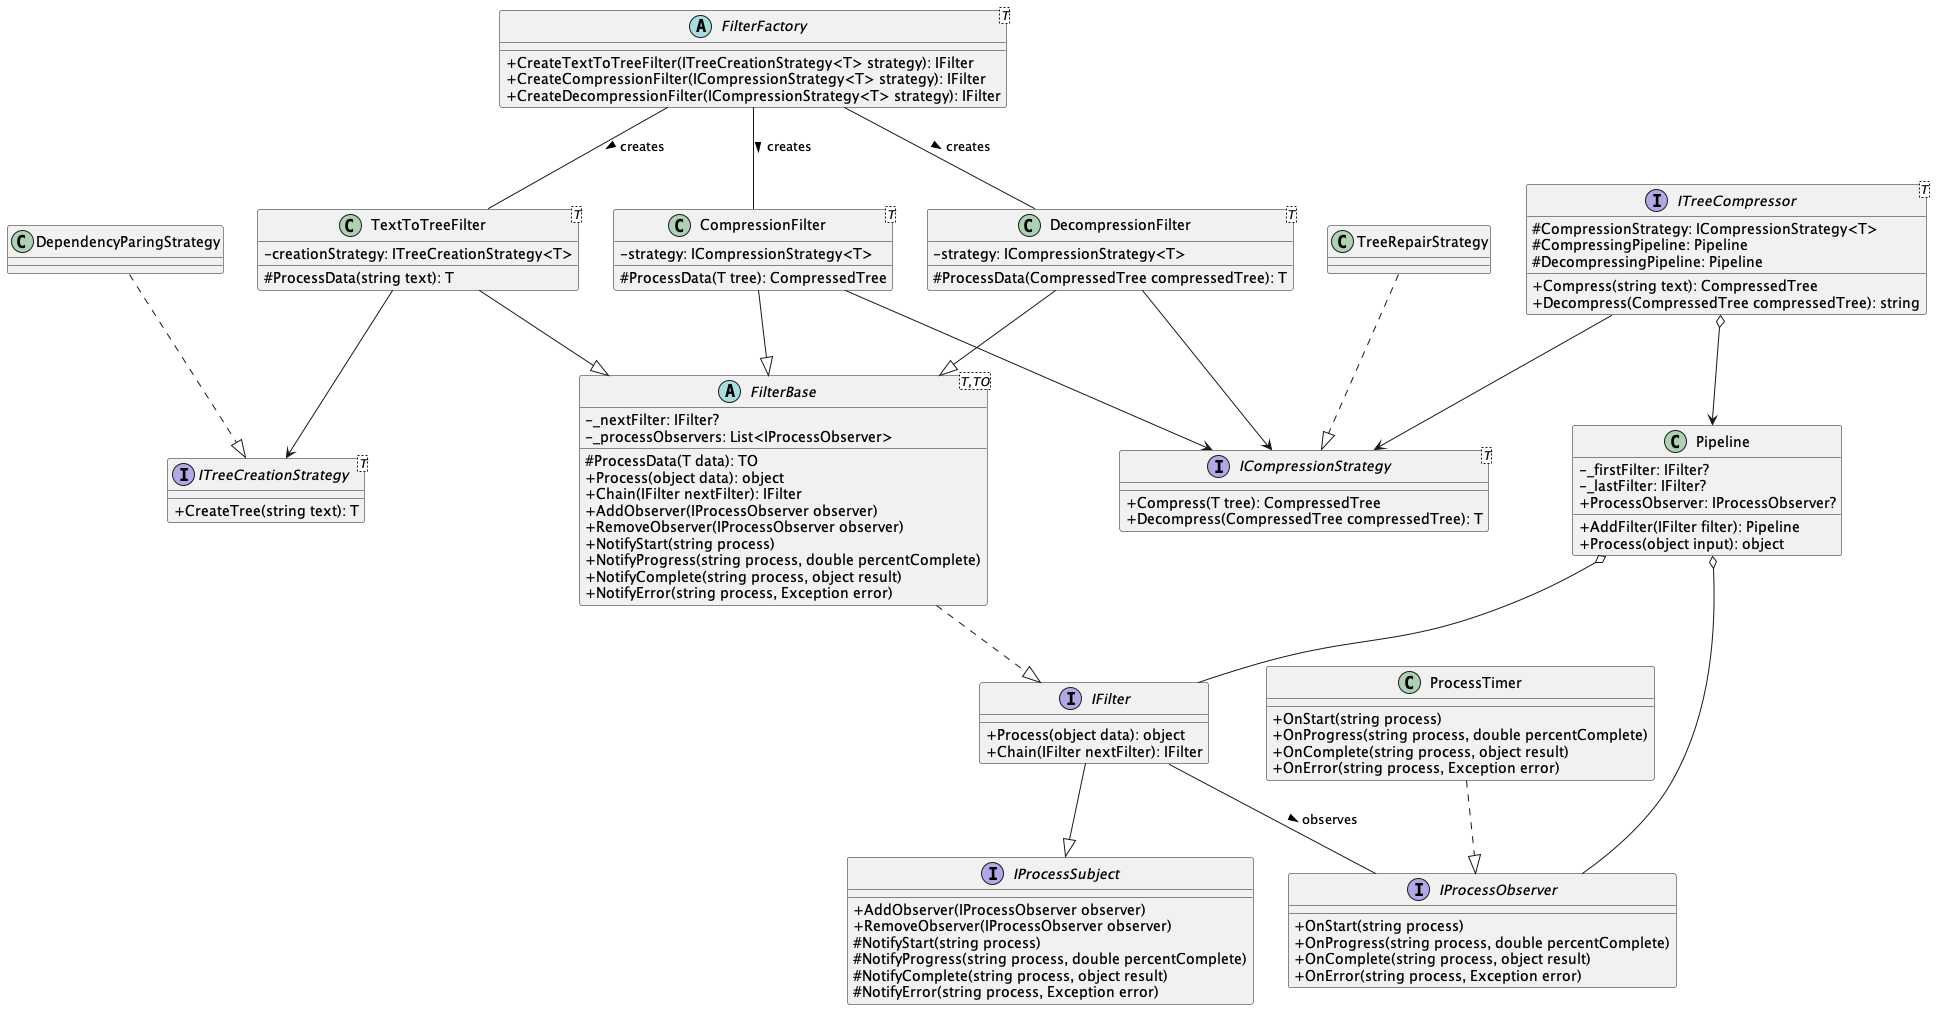
\includegraphics[width=\textwidth]{fig/class-diagram.png}
        \caption{Třídní diagram části implementace zaměření na řetězení filtrů}
        \label{fig:class-diagram}
    \end{figure}
\end{frame}

\section{Algoritmy}
\begin{frame}{Algoritmy}
  
  
\end{frame}

\end{document}